% \documentclass[lineno,twocolumn,endfloat,biblatex]{biophys-new}
\documentclass{biophys-new}
\usepackage[utf8]{inputenc}
\usepackage{graphicx}
\usepackage[colorlinks,allcolors=cyan!70!black]{hyperref}
\usepackage{glossaries}
\usepackage{textcomp}
% Uncomment if using biblatex
% \addbibresource{sample.bib}
\newacronym{nka}{NKA}{sodium-potassium ATPase pump}
\title{Model comparison and system analysis of Na+/K+-ATPase using bond graph}
\runningtitle{Biophysical Journal Template} %% For page header

\author[1,*]{First author}
\author[2]{Second author}
\runningauthor{Author1 and Author2} %% For page header

\affil[1]{Institution A, Address A}
\affil[2]{Institution B, Address B}

\corrauthor[*]{abx@xyz.edu}

% \papertype{Letters}
\papertype{Article}
% \papertype{Computational Tools}


\begin{document}

\begin{frontmatter}

\begin{abstract}
Each manuscript must be accompanied by an informative abstract of no more than 300 words. Abstracts should describe the substance of the manuscript in language non-specialists can understand, and must make clear the biological significance of the research. Reference citations are not allowed in the Abstract of a manuscript. 
\end{abstract}

\begin{sigstatement}
Each manuscript must also have a statement of significance or no more than 120 words. Each manuscript must also have a statement of significance or no more than 120 words. Each manuscript must also have a statement of significance or no more than 120 words.
\end{sigstatement}
\end{frontmatter}

\section*{Introduction}

The \gls{nka} uses the hydrolysis of ATP to move Na\textsuperscript{+} ions out of the cell and K\textsuperscript{+} ions into the cell,
in both cases against steep concentration gradients. ATP hydrolysis can be thought of as the energy source that tops up the cell's `sodium' battery,
since the the majority of transmembrane transport processes are driven by this sodium gradient.
The NKA pump is therefore critical to cellular function in all cell types.

In this paper we use a bond graph approach to examine a number of models of NKA in which mass, charge and energy are each conserved.
We examine a previously published 15-state bond graph model,
and then show how a much simpler 6-state model captures the biophysics of the pump, matches experimental data.
We then use the bond graph to examine the energy expenditure of the \Gls{nka}p and energy storage under different conditions.

\subsection*{\Gls{nka} physiology and models}

The \Gls{nka} was discovered in 1957\cite{skou_influence_1957},
and is a chemical molecular machine responsible for the movement of Na\textsuperscript{+} and K\textsuperscript{+} ions across the cell membrane against their concentration gradients.
The Albers–Post kinetic scheme \cite{albers_role_1963,post_activation_1972} was proposed to describe the transport mechanism of the \Gls{nka} \cite{apell_electrogenic_1989},
where the \Gls{nka} undergoes Na\textsuperscript{+}-dependent phosphorylation and K\textsuperscript{+}-dependent dephosphorylation reactions and alternates between two main conformations, 
\textit{E1} and \textit{E2}, which expose the transport sites to the intracellular and extracellular sides of the membrane, respectively.

Many intermediate conformational states and partial reaction steps have been proposed \cite{post_flexibility_1969,karlish_conformational_1978,glynn_na_1985, apell_electrogenic_1989,terkildsen_balance_2007},
while structural studies have provided insights into the molecular mechanism of the \Gls{nka}.
The cryo-electron microscopy (cryo-EM) structures of \Gls{nka} in different conformational states were reported,
including exoplasmic side-open (\textit{E2\textperiodcentered P})\cite{kanai_binding_2021,nguyen_structural_2022},
K\textsuperscript{+}-occluded (\textit{E2\textperiodcentered [2K] \textperiodcentered Pi}) \cite{morth_crystal_2007,shinoda_crystal_2009,nguyen_structural_2022},
(\textit{E2\textperiodcentered [2K]})\cite{guo_cryo-em_2022},
cytoplasmic side-open (\textit{E1})\cite{nguyen_structural_2022}, ATP bound cytoplasmic side-open (\textit{E1\textperiodcentered ATP})\cite{nguyen_structural_2022},
(\textit{E1\textperiodcentered [3Na]\textperiodcentered ATP})\cite{guo_cryo-em_2022}.
Na\textsuperscript{+}-occluded (\textit{E1\textperiodcentered [3Na]\textperiodcentered P\text{-}ADP}) \cite{nyblom_crystal_2013,kanai_crystal_2013,nguyen_structural_2022},
and (\textit{E1\textperiodcentered [3Na]})\cite{guo_cryo-em_2022}.

Since the \Gls{nka} transports three Na\textsuperscript{+} ions outward and two K\textsuperscript{+} ions inward,
the process gives rise to a net outward current and is therefore electrogenic\cite{apell_electrogenic_1989,glitsch_electrophysiology_2001}.
That is, the \Gls{nka} contributes to the membrane potential and the transport rate is a function of the membrane potential.
The electrogenicity of the \Gls{nka} has been studied experimentally and the main voltage-dependent steps are associated with the binding and release of Na\textsuperscript{+} ions.
These include Na\textsuperscript{+}-mediated transient electrical currents \cite{nakao_voltage_1986} and Na\textsuperscript{+} efflux \cite{gadsby_extracellular_1993}.
More recently, the electrogenicity of extracellular K\textsuperscript{+} binding was also investigated \cite{peluffo_electrogenic_1997}
while K\textsuperscript{+} uptake was found to be less voltage-dependent \cite{moreno_transient_2020}.

Terkildsen et al. \cite{terkildsen_balance_2007} developed a kinetic model of the \Gls{nka} based on the Albers-Post scheme including fifteen intermediate states.
This model detailed the binding and release of Na\textsuperscript{+} and K\textsuperscript{+} ions and their voltage dependence.
It also explicitly included the proton to enable the study of the effect of pH on the pump function,
which was found to be significant in ischemic conditions.
The model was subsequently corrected by Pan et al. \cite{pan_cardiac_2020} to address inconsistencies in the original model,
and re-parameterised to ensure thermodynamic consistency using a bond graph.
The \Gls{nka} is responsible for 9\% of myocardial energy expenditure during contraction and 17\% at rest \cite{schramm1994energy},
so it is important to guarantee thermodynamic consistency.
Hence, the bond graph is also used in this study to facilitate energy-based analysis.
The reduction of free energy available from ATP hydrolysis results in an accumulation of intracellular Na\textsuperscript{+} ions \cite{jansen2003energy},
while increase in intracellular Pi and decreases in intracellular pH and ATP were associated with ischemic conditions \cite{huang1984regulation}.

\subsection*{Bond graph basics}

This paper builds on a previous publication {[}.{]} where we developed
models of transmembrane glucose transport using facilitated diffusion
with the GLUT2 transporter and sodium-driven glucose cotransport with
the electrogenic SGLT2 transporter. These models were also developed
using bond graph methods to ensure thermodynamic consistency
(conservation of mass, conservation of charge and conservation of
energy) but for convenience we begin with a summary of the bond graph
approach that underpins all subsequent analysis.


\section*{Methods}


\subsection*{Bond graph model of \Gls{nka} with 15 states}


\cite{pan_cardiac_2020}

% include 15state_eqs.tex to get the equations
The equations for conservation of mass are expressed as below.
\begin{align*}
\frac{d q_m^1}{dt}&=v_m^{15}-v_m^{1}      &  \frac{d q_m^2}{dt} &=v_m^{1}-v_m^{2}   &  \frac{d q_m^3}{dt}&=v_m^{2}-v_m^{3}\\
\frac{d q_m^4}{dt}&=v_m^{3}-v_m^{4}       &  \frac{d q_m^5}{dt} &=v_m^{4}-v_m^{5}    &  \frac{d q_m^6}{dt}&=v_m^{5}-v_m^{6}\\
\frac{d q_m^7}{dt}&=v_m^{6}-v_m^{7}       &  \frac{d q_m^8}{dt} &=v_m^{7}-v_m^{8}    &  \frac{d q_m^9}{dt}&=v_m^{8}-v_m^{9} \\
\frac{d q_m^{10}}{dt}&=v_m^{9}-v_m^{10}   &  \frac{d q_m^{11}}{dt}&=v_m^{10}-v_m^{11} &  \frac{d q_m^{12}}{dt}&=v_m^{11}-v_m^{12}\\
\frac{d q_m^{13}}{dt}&=v_m^{12}-v_m^{13}  &  \frac{d q_m^{14}}{dt}&=v_m^{13}-v_m^{14} &  \frac{d q_m^{15}}{dt}&=v_m^{14}-v_m^{15}\\
\end{align*}

The chemical potentials are given by the following.

\begin{align*}
\mu_m^1 & = RT\ln(K_1q_m^1) & \mu_m^2 & = RT\ln(K_2q_m^2) & \mu_m^3 & = RT\ln(K_3q_m^3) & \mu_m^4 & = RT\ln(K_4q_m^4) & \mu_m^5 & = RT\ln(K_5q_m^5) \\
\mu_m^6 & = RT\ln(K_6q_m^6) & \mu_m^7 & = RT\ln(K_7q_m^7) & \mu_m^8 & = RT\ln(K_8q_m^8) & \mu_m^9 & = RT\ln(K_9q_m^9) & \mu_m^{10} & = RT\ln(K_{10}q_m^{10}) \\
\mu_m^{11} & = RT\ln(K_{11}q_m^{11}) & \mu_m^{12} & = RT\ln(K_{12}q_m^{12}) & \mu_m^{13} & = RT\ln(K_{13}q_m^{13}) & \mu_m^{14} & = RT\ln(K_{14}q_m^{14}) & \mu_m^{15} & = RT\ln(K_{15}q_m^{15})
\end{align*}

\begin{align*}
\mu_i^{K+} & = RT\ln(K_i^Kq_i^{K+}) & \mu_i^{Na+} & = RT\ln(K_i^{Na}q_i^{Na+}) & \mu_o^{Na+} & = RT\ln(K_o^{Na}q_o^{Na+}) & \mu_o^{K+} & = RT\ln(K_o^Kq_o^{K+})\\
\mu_i^{ATP} & = RT\ln(K_i^{ATP}q_i^{ATP}) & \mu_i^{ADP} & = RT\ln(K_i^{ADP}q_i^{ADP}) & \mu_i^{P_i} & = RT\ln(K_i^{P_i}q_i^{P_i}) & \mu_i^{H} & = RT\ln(K_i^{H}q_i^{H}) \\
\end{align*}

The flow rates are given by:

\begin{alignat*}{2}
v_m^{1}  &= \kappa_1 \left( K_1 q_m^1 - K_2 q_m^2 K_i^{K} q_i^{K+} \right)
&\qquad
v_m^{2}  &= \kappa_2 \left( K_2 q_m^2 - K_3 q_m^3 K_i^{K} q_i^{K+} \right) \\[6pt]
v_m^{3}  &= \kappa_3 \left( K_3 q_m^3 K_i^{Na} q_i^{Na+} - K_4 q_m^4 \right)
&\qquad
v_m^{4}  &= \kappa_4 \left( K_4 q_m^4 K_i^{Na} q_i^{Na+} - K_5 q_m^5 \right) \\[6pt]
v_m^{5}  &= \kappa_5 \left( K_5 q_m^5 K_i^{Na} q_i^{Na+}
            - K_6 q_m^6 \exp\left( \frac{z_1 F u_m^e}{RT} \right) \right)
&\qquad
v_m^{6}  &= \kappa_6 \left( K_6 q_m^6 - K_7 q_m^7 K_i^{ADP} q_i^{ADP} \right) \\[6pt]
v_m^{7}  &= \kappa_7 \left( K_7 q_m^7 - K_8 q_m^8 \right)
&\qquad
v_m^{8}  &= \kappa_8 \left( K_8 q_m^8 - K_9 q_m^9 K_o^{Na} q_o^{Na+}
             \exp\left( \frac{z_1 F u_m^e}{RT} \right) \right) \\[6pt]
v_m^{9}  &= \kappa_9 \left( K_9 q_m^9 - K_{10} q_m^{10} K_o^{Na} q_o^{Na+} \right)
&\qquad
v_m^{10} &= \kappa_{10} \left( K_{10} q_m^{10} - K_{11} q_m^{11} K_o^{Na} q_o^{Na+} \right) \\[6pt]
v_m^{11} &= \kappa_{11} \left( K_{11} q_m^{11} K_o^{K} q_o^{K+} - K_{12} q_m^{12} \right)
&\qquad
v_m^{12} &= \kappa_{12} \left( K_{12} q_m^{12} K_o^{K} q_o^{K+} - K_{13} q_m^{13} \right) \\[6pt]
v_m^{13} &= \kappa_{13} \left( K_{13} q_m^{13}
             - K_{14} q_m^{14} K_i^{P_i} q_i^{P_i} K_i^{H} q_i^{H} \right)
&\qquad
v_m^{14} &= \kappa_{14} \left( K_{14} q_m^{14} K_i^{ATP} q_i^{ATP}
             - K_{15} q_m^{15} \right) \\[6pt]
v_m^{15} &= \kappa_{15} \left( K_{15} q_m^{15} - K_{16} q_m^{16} \right)
& &
\end{alignat*}

\begin{figure}
\caption{15-state model, adapted from \cite{pan_cardiac_2020}.}
\centering
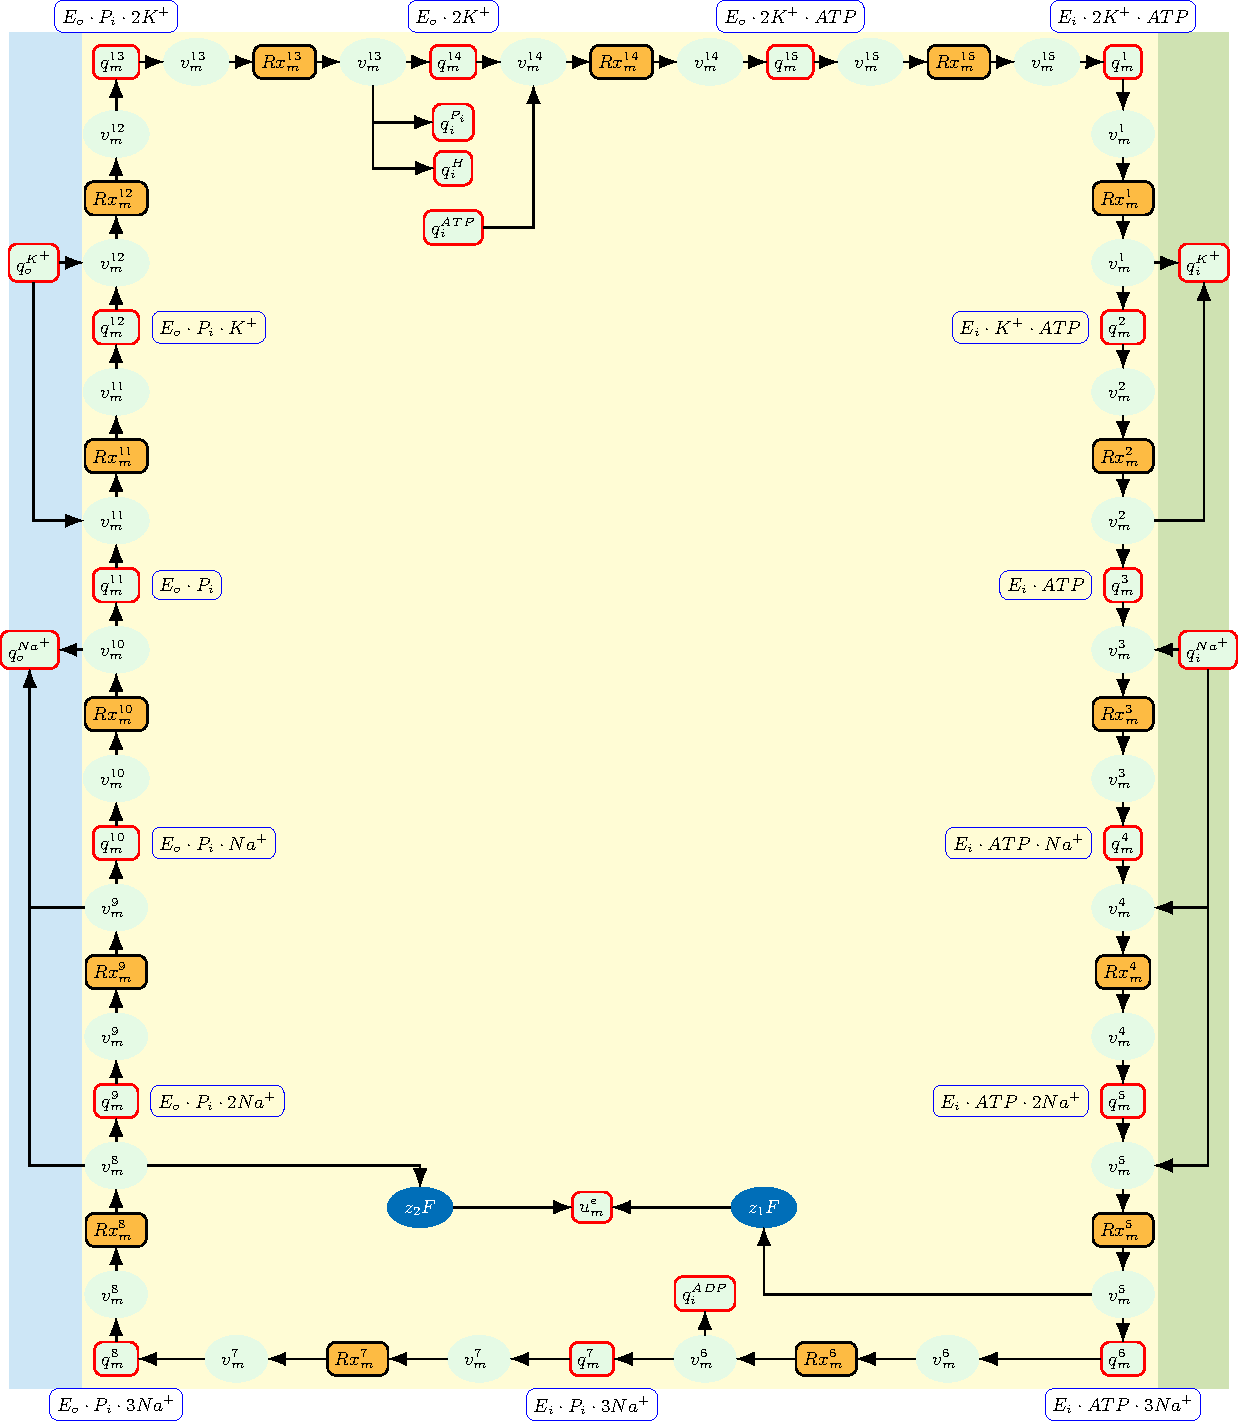
\includegraphics[width=1\linewidth]{15state.pdf}
\end{figure}

\subsection*{6-state model and parameter fitting}

We build a 6-state model, in Figure \ref{fig:6state}, based on the scheme in Fig. 1b of \cite{nguyen_structural_2022} with slight modifications.
We merged (\textit{E1\textperiodcentered [3Na]\textperiodcentered ATP}) and (\textit{E1\textperiodcentered [3Na]\textperiodcentered P\text{-}ADP}), 
while splitting the release of ADP AND Na\textsuperscript{+} into two steps.
\begin{figure}
\caption{6-state model.}
      \label{fig:6state}
\centering
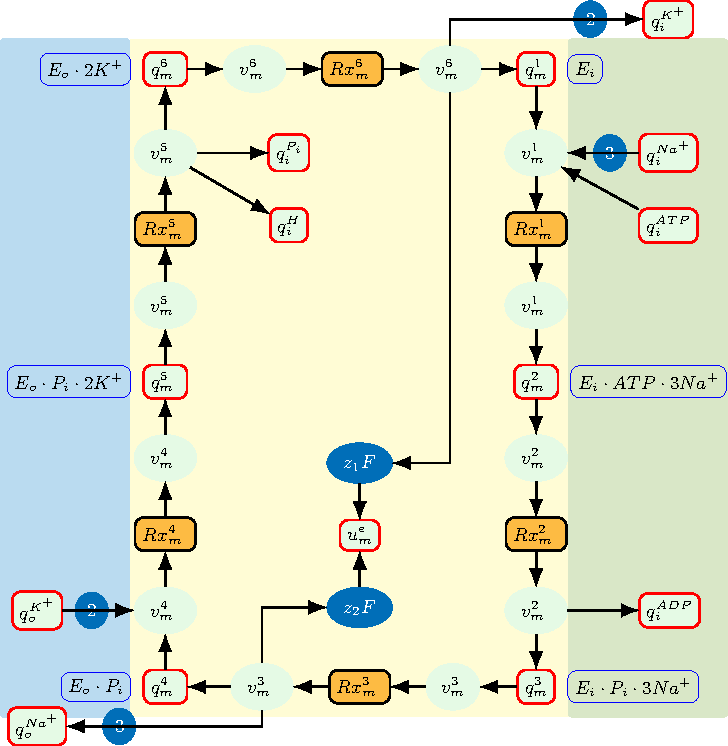
\includegraphics[width=0.7\linewidth]{6state_1.pdf}
\end{figure}

The equations for conservation of mass are expressed as below.
\begin{align*}
\frac{d q_m^1}{dt}&=v_m^{6}-v_m^{1}      &  \frac{d q_m^2}{dt} &=v_m^{1}-v_m^{2}   &  \frac{d q_m^3}{dt}&=v_m^{2}-v_m^{3}\\
\frac{d q_m^4}{dt}&=v_m^{3}-v_m^{4}       &  \frac{d q_m^5}{dt} &=v_m^{4}-v_m^{5}    &  \frac{d q_m^6}{dt}&=v_m^{5}-v_m^{6}\\
\end{align*}

The chemical potentials are given by the following.

\begin{align*}
\mu_m^1 & = RT\ln(K_1q_m^1) & \mu_m^2 & = RT\ln(K_2q_m^2) & \mu_m^3 & = RT\ln(K_3q_m^3)  \\
\mu_m^4 & = RT\ln(K_4q_m^4) & \mu_m^5 & = RT\ln(K_5q_m^5) & \mu_m^6 & = RT\ln(K_6q_m^6) 
\end{align*}

\begin{align*}
\mu_i^{K+} & = RT\ln(K_i^Kq_i^{K+}) & \mu_i^{Na+} & = RT\ln(K_i^{Na}q_i^{Na+}) & \mu_o^{Na+} & = RT\ln(K_o^{Na}q_o^{Na+}) & \mu_o^{K+} & = RT\ln(K_o^Kq_o^{K+})\\
\mu_i^{ATP} & = RT\ln(K_i^{ATP}q_i^{ATP}) & \mu_i^{ADP} & = RT\ln(K_i^{ADP}q_i^{ADP}) & \mu_i^{P_i} & = RT\ln(K_i^{P_i}q_i^{P_i}) & \mu_i^{H} & = RT\ln(K_i^{H}q_i^{H}) \\
\end{align*}

The flow rates are given by:

\begin{alignat*}{2}
v_m^1 &= \kappa_1\left( K_1 q_m^1 (K_i^{Na} q_i^{Na+})^3 K_i^{ATP} q_i^{ATP}
         - K_2 q_m^2 \right)
&\qquad
v_m^2 &= \kappa_2\left( K_2 q_m^2
         - K_3 q_m^3 K_i^{ADP} q_i^{ADP} \right) \\[6pt]
v_m^3 &= \kappa_3\left( K_3 q_m^3
         - K_4 q_m^4 (K_o^{Na} q_o^{Na+})^3
         \exp\left( \frac{z_2 F u_m^e}{RT} \right)\right)
&\qquad
v_m^4 &= \kappa_4\left( K_4 q_m^4 (K_o^{K} q_o^{K+})^2
         - K_5 q_m^5 \right) \\[6pt]
v_m^5 &= \kappa_5\left( K_5 q_m^5
         - K_6 q_m^6 K_i^{P_i} q_i^{P_i} K_i^{H} q_i^{H} \right)
&\qquad
v_m^6 &= \kappa_6\left( K_6 q_m^6
         - K_7 q_m^7 (K_i^{K} q_i^{K+})^2
         \exp\left( \frac{z_1 F u_m^e}{RT} \right)\right)
\end{alignat*}



Figure \ref{fig:6state_v3} shows a 6-state model with voltage dependence in the Na binding step.
\begin{figure}
\caption{6-state model with voltage dependence in the Na binding step.}
\label{fig:6state_v3}
\centering
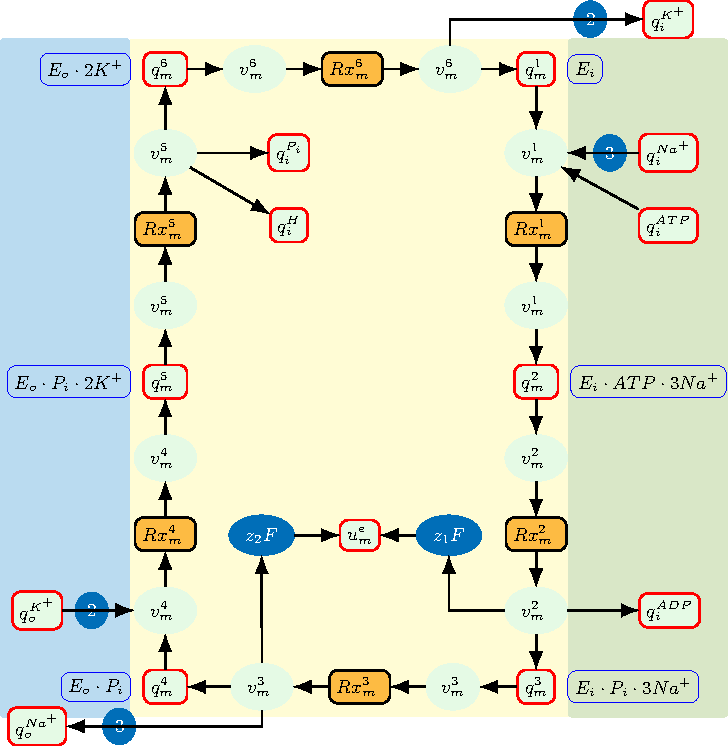
\includegraphics[width=0.7\linewidth]{6state_3.pdf}
\end{figure}

The equations for conservation of mass are expressed as below.
\begin{align*}
\frac{d q_m^1}{dt}&=v_m^{6}-v_m^{1}      &  \frac{d q_m^2}{dt} &=v_m^{1}-v_m^{2}   &  \frac{d q_m^3}{dt}&=v_m^{2}-v_m^{3}\\
\frac{d q_m^4}{dt}&=v_m^{3}-v_m^{4}       &  \frac{d q_m^5}{dt} &=v_m^{4}-v_m^{5}    &  \frac{d q_m^6}{dt}&=v_m^{5}-v_m^{6}\\
\end{align*}

The chemical potentials are given by the following.

\begin{align*}
\mu_m^1 & = RT\ln(K_1q_m^1) & \mu_m^2 & = RT\ln(K_2q_m^2) & \mu_m^3 & = RT\ln(K_3q_m^3)  \\
\mu_m^4 & = RT\ln(K_4q_m^4) & \mu_m^5 & = RT\ln(K_5q_m^5) & \mu_m^6 & = RT\ln(K_6q_m^6) 
\end{align*}

\begin{align*}
\mu_i^{K+} & = RT\ln(K_i^Kq_i^{K+}) & \mu_i^{Na+} & = RT\ln(K_i^{Na}q_i^{Na+}) & \mu_o^{Na+} & = RT\ln(K_o^{Na}q_o^{Na+}) & \mu_o^{K+} & = RT\ln(K_o^Kq_o^{K+})\\
\mu_i^{ATP} & = RT\ln(K_i^{ATP}q_i^{ATP}) & \mu_i^{ADP} & = RT\ln(K_i^{ADP}q_i^{ADP}) & \mu_i^{P_i} & = RT\ln(K_i^{P_i}q_i^{P_i}) & \mu_i^{H} & = RT\ln(K_i^{H}q_i^{H}) \\
\end{align*}

The flow rates are given by:

\begin{alignat*}{2}
v_m^1 &= \kappa_1\left( K_1 q_m^1 (K_i^{Na} q_i^{Na+})^3 K_i^{ATP} q_i^{ATP}
         - K_2 q_m^2 \right)
&\qquad
v_m^2 &= \kappa_2\left( K_2 q_m^2
         - K_3 q_m^3 K_i^{ADP} q_i^{ADP} \exp\left( \frac{z_1 F u_m^e}{RT} \right)\right) \\[6pt]
v_m^3 &= \kappa_3\left( K_3 q_m^3
         - K_4 q_m^4 (K_o^{Na} q_o^{Na+})^3
         \exp\left( \frac{z_2 F u_m^e}{RT} \right)\right)
&\qquad
v_m^4 &= \kappa_4\left( K_4 q_m^4 (K_o^{K} q_o^{K+})^2
         - K_5 q_m^5 \right) \\[6pt]
v_m^5 &= \kappa_5\left( K_5 q_m^5
         - K_6 q_m^6 K_i^{P_i} q_i^{P_i} K_i^{H} q_i^{H} \right)
&\qquad
v_m^6 &= \kappa_6\left( K_6 q_m^6
         - K_7 q_m^7 (K_i^{K} q_i^{K+})^2
         \right)
\end{alignat*}

The constraint on the thermodynamicparameters of reaction $Rx_m^1$ is as follows:
\begin{equation}
      \label{eq:constraint_ATPNai_3}
\dfrac{K_1W_i(K_i^{Na}W_i)^3K_i^{ATP}W_i}{K_2W_i} = \dfrac{1}{(K_{d,Na_i})^2 K_{d,Na_i}^0K_{d,ATP}}
\end{equation}
where $K_{d,Na_i}$ and $K_{d,Na_i}^0$ are voltage-independent dissociation constant and voltage-dependent dissociation constant of intracellular sodium respectively,
$K_{d,ATP}$ is the dissociation constant of intracellular ATP.

The constraint on the parameters of reaction $Rx_m^3$ is as follows:
\begin{equation}
      \label{eq:constraint_Nao_3}
\dfrac{K_3W_i}{K_4W_o(K_o^{Na}W_o)^3} = \dfrac{(K_{d,Na_o})^2K_{d,Na_o}^0}{1}
\end{equation}
where $K_{d,Na_o}$ are voltage-independent dissociation constant of extracellular sodium.

The constraint on the parameters of reaction $Rx_m^4$ is as follows:
\begin{equation}
      \label{eq:constraint_Ko_3}
\dfrac{K_4W_o(K_o^{K}W_o)^2}{K_5W_o} = \dfrac{1}{(K_{d,K_o})^2}
\end{equation}
where $K_{d,K_o}$ is the dissociation constant of extracellular potassium.

The constraint on the parameters of reaction $Rx_m^6$ is as follows:
\begin{equation}
      \label{eq:constraint_Ki_3}
\dfrac{K_6W_o}{K_1W_i(K_i^{K}W_i)^2} = \dfrac{(K_{d,K_i})^2}{1}
\end{equation}
where $K_{d,K_i}$ is the dissociation constant of intracellular potassium.



% include 6state_eqs.tex to get the equations
We build a 6-state model, in Figure \ref{fig:6state_v2}, based on the proposed scheme in the supplmental material of \cite{nguyen_structural_2022} using bond graph approach.
\begin{figure}
\caption{6-state model, based on the proposed scheme in \cite{nguyen_structural_2022}.}
\label{fig:6state_v2}
\centering
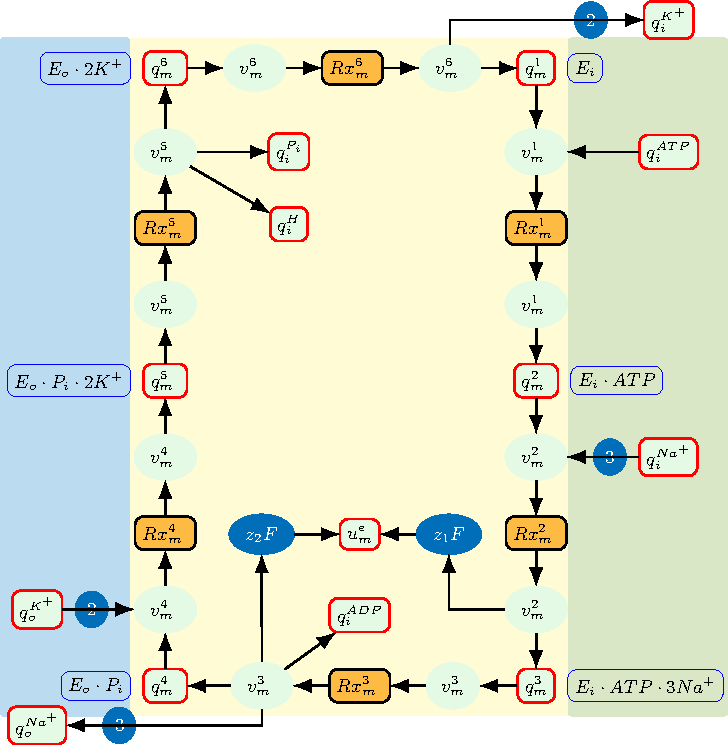
\includegraphics[width=0.7\linewidth]{6state_2.pdf}
\end{figure}

The equations for conservation of mass are expressed as below.
\begin{align*}
\frac{d q_m^1}{dt}&=v_m^{6}-v_m^{1}      &  \frac{d q_m^2}{dt} &=v_m^{1}-v_m^{2}   &  \frac{d q_m^3}{dt}&=v_m^{2}-v_m^{3}\\
\frac{d q_m^4}{dt}&=v_m^{3}-v_m^{4}       &  \frac{d q_m^5}{dt} &=v_m^{4}-v_m^{5}    &  \frac{d q_m^6}{dt}&=v_m^{5}-v_m^{6}\\
\end{align*}

The chemical potentials are given by the following.

\begin{align*}
\mu_m^1 & = RT\ln(K_1q_m^1) & \mu_m^2 & = RT\ln(K_2q_m^2) & \mu_m^3 & = RT\ln(K_3q_m^3)  \\
\mu_m^4 & = RT\ln(K_4q_m^4) & \mu_m^5 & = RT\ln(K_5q_m^5) & \mu_m^6 & = RT\ln(K_6q_m^6) 
\end{align*}

\begin{align*}
\mu_i^{K+} & = RT\ln(K_i^Kq_i^{K+}) & \mu_i^{Na+} & = RT\ln(K_i^{Na}q_i^{Na+}) & \mu_o^{Na+} & = RT\ln(K_o^{Na}q_o^{Na+}) & \mu_o^{K+} & = RT\ln(K_o^Kq_o^{K+})\\
\mu_i^{ATP} & = RT\ln(K_i^{ATP}q_i^{ATP}) & \mu_i^{ADP} & = RT\ln(K_i^{ADP}q_i^{ADP}) & \mu_i^{P_i} & = RT\ln(K_i^{P_i}q_i^{P_i}) & \mu_i^{H} & = RT\ln(K_i^{H}q_i^{H}) \\
\end{align*}

The flow rates are given by:

\begin{alignat*}{2}
v_m^1 &= \kappa_1\left( K_1 q_m^1 K_i^{ATP} q_i^{ATP}
         - K_2 q_m^2 \right)
&\qquad
v_m^2 &= \kappa_2\left( K_2 q_m^2 (K_i^{Na} q_i^{Na+})^3
         - K_3 q_m^3 
         \exp\left( \frac{z_1 F u_m^e}{RT} \right) \right) \\[6pt]
v_m^3 &= \kappa_3\left( K_3 q_m^3
         - K_4 q_m^4 (K_o^{Na} q_o^{Na+})^3 K_i^{ADP} q_i^{ADP}
         \exp\left( \frac{z_2 F u_m^e}{RT} \right)\right)
&\qquad
v_m^4 &= \kappa_4\left( K_4 q_m^4 (K_o^{K} q_o^{K+})^2
         - K_5 q_m^5 \right) \\[6pt]
v_m^5 &= \kappa_5\left( K_5 q_m^5
         - K_6 q_m^6 K_i^{P_i} q_i^{P_i} K_i^{H} q_i^{H} \right)
&\qquad
v_m^6 &= \kappa_6\left( K_6 q_m^6
         - K_7 q_m^7 (K_i^{K} q_i^{K+})^2\right)
\end{alignat*}

The constraint on the thermodynamicparameters of reaction $Rx_m^1$ is as follows:

\begin{equation}
      \label{eq:constraint_ATP_2}
\dfrac{K_1W_iK_i^{ATP}W_i}{K_2W_i} = \dfrac{1}{K_{d,ATP}}
\end{equation}
where $K_{d,ATP}$ is the dissociation constant of intracellular ATP.

\begin{equation}
      \label{eq:constraint_Nai_2}
\dfrac{K_2W_i(K_i^{Na+}W_i)^3}{K_3W_i} = \dfrac{1}{(K_{d,Na_i})^2 K_{d,Na_i}^0}
\end{equation}
where $K_{d,Na_i}$ and $K_{d,Na_i}^0$ are voltage-independent dissociation constant and voltage-dependent dissociation constant of intracellular sodium respectively.

The constraint on the parameters of reaction $Rx_m^3$ is as follows:
\begin{equation}
      \label{eq:constraint_Nao_2}
\dfrac{K_3W_i}{K_4W_o(K_o^{Na+}W_o)^3} = \dfrac{(K_{d,Na_o})^2K_{d,Na_o}^0}{1}
\end{equation}
where $K_{d,Na_o}$ are voltage-independent dissociation constant of extracellular sodium.

The constraint on the parameters of reaction $Rx_m^4$ is as follows:
\begin{equation}
      \label{eq:constraint3_Ko_2}
\dfrac{K_4W_o(K_o^{K+}W_o)^2}{K_5W_o} = \dfrac{1}{(K_{d,K_o})^2}
\end{equation}
where $K_{d,K_o}$ is the dissociation constant of extracellular potassium.

The constraint on the parameters of reaction $Rx_m^6$ is as follows:
\begin{equation}
      \label{eq:constraint4_Ki_2}
\dfrac{K_6W_o}{K_1W_i(K_i^{K+}W_i)^2} = \dfrac{(K_{d,K_i})^2}{1}
\end{equation}
where $K_{d,K_i}$ is the dissociation constant of intracellular potassium.




\subsubsection{Steady-state model and parameter fitting}

\subsubsection{Activity comparison }

\subsection*{Figures and Tables}



\begin{table}[hbt!]
\caption{An example table}
\label{tab:widgets}
\centering

\begin{threeparttable}

\begin{tabular}{c l r}
\hline
Code & Item & Quantity \\\hline
W1 & Widgets\tnote{a} & 42 \\
G35 & Gadgets & 13\tnote{b} \\
\hline
\end{tabular}

\begin{tablenotes}
\item[a] This is a table note.
\item[b] This is another table note.
\end{tablenotes}

\end{threeparttable}

\end{table}

\begin{figure}[hbt!]
\centering
\includegraphics[width=0.6\linewidth]{example-image}
\caption{A figure example.}
\label{fig:view}

\end{figure}

\section*{Results}

\LaTeX{} is great at typesetting mathematics:

Let $X_1, X_2, \ldots, X_n$ be a sequence of independent and identically distributed random variables with $\text{E}[X_i] = \mu$ and $\text{Var}[X_i] = \sigma^2 < \infty$, and let
\begin{equation}
\label{eq:CLT}
S_n = \frac{X_1 + X_2 + \cdots + X_n}{n}
      = \frac{1}{n}\sum_{i}^{n} X_i
\end{equation}
denote their mean. Then as $n$ approaches infinity, the random variables $\sqrt{n}(S_n - \mu)$ converge in distribution to a normal $\mathcal{N}(0, \sigma^2)$. Thus concludes the explanation about Eq.~\ref{eq:CLT}.


You can make lists with automatic numbering \dots

\begin{enumerate}
\item Like this,
\item and like this.
\end{enumerate}

\dots or bullet points \dots

\begin{itemize} 
\item Like this,
\item and like this.
\end{itemize}

\dots or with words and descriptions \dots

\begin{description}
\item[Word] Definition
\item[Concept] Explanation
\item[Idea] Text
\end{description}

An example quotation:

\begin{quote}
Lorem ipsum dolor sit amet, consectetur adipiscing elit, sed do eiusmod tempor incididunt ut labore et dolore magna aliqua. Ut enim ad minim veniam, quis nostrud exercitation ullamco laboris nisi ut aliquip ex ea commodo consequat.
\end{quote}


\section*{Discussion}


\section*{Conclusion}

Sed ut perspiciatis unde omnis iste natus error sit voluptatem accusantium doloremque laudantium, totam rem aperiam, eaque ipsa quae ab illo inventore veritatis et quasi architecto beatae vitae dicta sunt explicabo. 

\section*{Author Contributions}

Author1 designed the research. Author2 carried out all simulations, analyzed the data. Author1 and Author2 wrote the article. 

\section*{Acknowledgments}

We thank G. Harrison, B. Harper, and J. Doe for their help.

% Uncomment if using bibtex (default)
\bibliography{sample}

% Uncomment if using biblatex
% \printbibliography

\section*{Supplementary Material}

An online supplement to this article can be found by visiting BJ Online at \url{http://www.biophysj.org}.

\end{document}
